
\documentclass[fleqn,usenatbib]{rasti}

\usepackage{newtxtext,newtxmath}
\usepackage[T1]{fontenc}
\usepackage{graphicx}
\graphicspath{{./}{../}}
\usepackage{amsmath}
\usepackage{bm}
\usepackage{booktabs}
\usepackage{siunitx}

% ---- convenient shorthands (math mode only where needed) ----
\newcommand{\nHH}{n_{\mathrm{H_2}}}
\newcommand{\logn}{\log_{10}(n_{\mathrm{H_2}})}
\newcommand{\Gzero}{G_0}
\newcommand{\fshield}{f_{\mathrm{H_2}}}
\newcommand{\dex}{\,\text{dex}}
\newcommand{\Rsq}{R^2}
\newcommand{\Mratio}{\mathcal{M}}

% ============================================================
\title[Mass-accurate H\(_2\) surrogates at unseen UV field strengths]%
      {A mass-accurate machine-learning surrogate for molecular
       hydrogen density at unseen UV field strengths}

\author[D.~H.~Breger]{Daniel H.~Breger\(^{1}\)\thanks{E-mail: danielbreger@campus.technion.ac.il}
\\
\(^{1}\)Department of Physics, Technion,
Haifa, Israel}

\date{Accepted XXX. Received YYY; in original form ZZZ}
\pubyear{2026}

% ============================================================
\begin{document}

\label{firstpage}
\pagerange{\pageref{firstpage}--\pageref{lastpage}}
\maketitle

% ============================================================
\begin{abstract}
Can a machine-learning surrogate predict the molecular hydrogen density
field of an interstellar-medium simulation at a UV field strength it has
never seen --- accurately enough to trust the prediction as a
\emph{physical} field? We test this on seven \(128^3\) UV-only chemistry
simulations spanning \(\Gzero = 0.1\)--6.4 Habing, holding out one entire
simulation per fold and scoring predictions by H\(_2\) mass budget, bias,
and phase structure as well as log-space \(\Rsq\). Three ingredients
suffice: multi-scale box-filter neighbourhood features (a cheap shielding
proxy) halve the residual scatter of tabular models; density-weighted
training and a mass-weighted bias calibration, fitted on training cubes
alone, remove a \(+0.3\dex\) systematic offset that would otherwise
inflate the H\(_2\) mass by 70--90 per cent. The resulting pipeline
attains RMSE \(=0.25\dex\), \(\Rsq = 0.990\), and total H\(_2\) mass within
9 per cent on every held-out fold. A 3D U-Net is more accurate when
interpolating but over-predicts the mass of the hardest extrapolation
fold by more than two orders of magnitude --- a failure invisible to
\(\Rsq\), which separates the two models by only 0.02. Physically scored,
out-of-distribution reliability is set by input representation and
calibration, not architecture.
\end{abstract}
\begin{keywords}
ISM: molecules -- ISM: clouds -- astrochemistry --
methods: numerical -- methods: statistical
\end{keywords}

% ============================================================
\section{Introduction}
\label{sec:intro}

The H\(_2\) abundance sets the initial conditions of star formation, but
computing it self-consistently in a three-dimensional simulation means
integrating stiff non-equilibrium chemistry --- grain-surface formation
\citep{Cazaux2004}, Lyman--Werner photodissociation
\citep{Habing1968,Draine1996}, and self-shielding
\citep{Wolcott-Green2011} --- in every cell, a cost that limits
resolution and parameter coverage \citep{Grassi2014}. Machine-learned
emulators of ISM chemistry
\citep{deMijolla2019,Palud2023,Holdship2021,Grassi2022,Branca2024,Janssen2026}
replace the solver with a fast local mapping, but they are
zero-dimensional --- each cell is treated independently --- while the
equilibrium \(\nHH\) of a cell depends on the shielding column of gas
around it, and they are conventionally scored by log-space error
statistics, while their downstream uses (mass budgets, phase statistics,
synthetic observations) consume the prediction as a physical field.

This paper asks one question: \emph{can a surrogate trained on
simulations at six UV field strengths predict the full \(\nHH\) field of a
seventh simulation, at a field strength absent from training, accurately
enough to be used as a physical field?} The question fixes the design.
Generalisation is measured by leave-one-\(\Gzero\)-out cross-validation
over a controlled seven-simulation UV sweep --- every fold withholds an
entire \(128^3\) cube. Success is measured by a metric hierarchy in which
the primary statistics are physical: the RMSE decomposed exactly into
bias and scatter, and the total H\(_2\) mass ratio; log-space \(\Rsq\) is
retained but demoted to a secondary statistic. Non-locality is treated
as a representation problem: we compare engineered multi-scale
neighbourhood features attached to tabular models (gradient-boosted
trees and multilayer perceptrons) against a volumetric 3D U-Net
\citep{Ronneberger2015,Cicek2016} that can learn shielding-like
aggregations through its receptive field.

The answer is yes, with qualifications that only the physical scoring
reveals. The best least-squares model carries a \(+0.32\dex\) systematic
offset on held-out cubes --- invisible at the precision \(\Rsq\) is
quoted, but a 70--90 per cent error in total H\(_2\) mass. Repairing it
requires treating the bias as a modelling target of its own: a
two-parameter, mass-weighted calibration fitted on training cubes alone
closes the mass budget in every fold. The U-Net, conversely, is the
best interpolator in the comparison and fails at both extrapolation
boundaries in a phase-localised, non-monotonic way that no global
calibration can repair. Section~\ref{sec:setup} describes the data,
protocol, and metrics; Section~\ref{sec:methods} the models;
Section~\ref{sec:results} the results; Section~\ref{sec:disc} what they
imply.

% ============================================================
\section{Data, protocol, and metrics}
\label{sec:setup}

\subsection{Simulation suite}
\label{sec:data}

The data are seven \(128^3\) uniform-grid simulations (14.7 million cells
in total) evolving identical turbulent ISM initial conditions under a
spatially uniform, time-steady UV field of strength
\(\Gzero \in \{0.1, 0.2, 0.4, 0.8, 1.6, 3.2, 6.4\}\) Habing, illuminating
each cube along \(+z\); the snapshots are quasi-equilibrium chemical
states. The suite is a controlled single-parameter sweep: the runs share
one turbulent realisation, so all generalisation claims concern the
UV-field axis alone (Section~\ref{sec:disc}), though the evolved
snapshots differ hydrodynamically as well as chemically (the median
temperature rises by an order of magnitude across the sweep). The target
\(\nHH\) spans \(\approx\)16 orders of magnitude and its per-cube mean
falls from \(-3.1\) to \(-7.2\) in \(\log_{10}\) as photodissociation
strengthens, so all modelling is done in \(\logn\) and each held-out cube
has a target distribution shifted relative to everything in training.

Each cell provides 15 input features: \(\log n_{\mathrm{H}}\), \(\log T\),
\(\log n_{\mathrm{H^+}}\), a dust-extinction proxy, \(\log\Gzero\), three
velocity and six face-centred magnetic-field components, and the
solver's H\(_2\) self-shielding factor \(\log\fshield\). The last is
special: it is a column integral over the very field being predicted,
computed by the solver the surrogate aims to replace, and would not be
available in deployment. We therefore quantify its contribution by
ablation (Section~\ref{sec:ablation}) and regard the configuration
without it as the deployable one.

\subsection{Protocol and metrics}
\label{sec:metrics}

All headline results use leave-one-\(\Gzero\)-out seven-fold
cross-validation; every model, tabular or volumetric, is scored on the
same native \(128^3\) cells of the held-out cube. Random cell-level
splits would put every \(\Gzero\) and the shared realisation in both
train and test --- a pointwise tree already exceeds \(\Rsq = 0.99\) there
--- and would say nothing about the intended use, prediction at an
unsimulated field strength. The two boundary folds (\(\Gzero = 0.1\),
6.4) require genuine extrapolation; the five interior folds require
interpolation. Single-cube transfer experiments confirm the protocol is
non-trivial: a model trained on one cube reaches mean \(\Rsq = 0.966\)
one geometric step away in \(\Gzero\) but only 0.888 at two steps and
essentially zero at the largest separations, so no training cube is
redundant.

\emph{Primary metrics.} The RMSE in \(\logn\), decomposed exactly as
\(\mathrm{RMSE}^2 = b^2 + s^2\) with \(b\) the mean residual (bias) and
\(s\) the residual scatter; and the total H\(_2\) mass ratio
\(\Mratio = \sum_i 10^{\hat y_i} / \sum_i 10^{y_i}\), the ratio of
predicted to true H\(_2\) mass on the uniform grid. A bias of \(b\) dex,
invisible to variance-normalised statistics, multiplies the mass budget
by up to \(10^{b}\).

\emph{Secondary metrics.} Log-space \(\Rsq\) (for comparability with the
emulator literature); phase-conditional \(\Rsq\) and bias for the
molecular (\(y > -4\)) and diffuse (\(y \le -4\)) populations, the
threshold lying between the two modes of the target distribution and the
conclusions insensitive to its placement within \([-5,-3]\); the fraction
\(f_{0.1}\) of cells within \(0.1\dex\); the mass-weighted MAE; the
Wasserstein distance \(W_1\) between predicted and true marginals; and a
skill score \(1 - \mathrm{MSE}/\mathrm{MSE_{XGB}}\) against the pointwise
gradient-boosted baseline. Folds, not cells, are the inferential unit;
cross-fold means carry the fold standard deviation, which bootstrap
resampling shows dominates the within-fold sampling uncertainty by an
order of magnitude.

Before exponentiation, predictions are clipped to within \(1\dex\) of the
held-out fold's true range so a handful of outlier cells cannot dominate
\(\Mratio\); for well-calibrated models the clip is never active, and
where it is we report \(\Mratio\) as a lower bound and flag it. Every
experiment writes a timestamped JSON log (configuration, seeds, per-fold
metrics, data checksum); tree results are bit-identical across runs.

% ============================================================
\section{Models}
\label{sec:methods}

\subsection{Spatial features, weighting, and calibration}
\label{sec:ingredients}

\emph{Multi-scale neighbourhood features.} To give per-cell models
access to spatial context we precompute box-filter averages of all 15
input fields at kernel widths \(k \in \{3,5,7\}\) voxels (reflected at
box faces), concatenated with the local features into a 60-dimensional
vector. The separable filter costs \(\mathcal{O}(N)\) per scale;
all 45 filtered fields for all seven cubes take \(\approx\)30\,s.
Averages of the column-type fields (density, extinction) act as crude
shielding estimators.

\emph{Density-weighted training.} The cell population is dominated by
diffuse gas while the H\(_2\) mass resides in the densest few per cent of
cells, so an unweighted log-space loss treats the mass-carrying tail as
an afterthought. Weighted variants use smooth exponential sample weights
rising from \(1\times\) at the 99th percentile of the training targets to
\(100\times\) at the 99.99th, normalised to unit mean.

\emph{Stacking and bias calibration.} A Ridge (\(\alpha = 1\))
meta-learner stacks the spatial-feature XGBoost and MLP, whose inductive
biases are complementary (bounded piecewise-constant extrapolation
versus smooth interpolation). Stacked predictions minimise squared error
but are not unbiased on an unseen \(\Gzero\)
(Section~\ref{sec:massbudget}), so for each fold we fit the
per-training-cube stack residual against \(\log\Gzero\) by two-parameter
least squares --- training-cube quantities only --- and subtract the
fitted value at the held-out \(\Gzero\). The residual functional is a
physical choice we evaluate explicitly: \emph{mean} calibration centres
the unweighted per-cube mean log residual; \emph{mass} calibration
centres the mass-weighted mean residual
\(b_M = \sum_i 10^{y_i}(\hat y_i - y_i)/\sum_i 10^{y_i}\), the constant
offset that approximately closes the total-mass budget (on the deployed
volumes it agrees with exact per-cube mass closure to within
\(0.018\dex\) in every fold).

\subsection{Model families}
\label{sec:models}

\emph{XGBoost} \citep{Chen2016}: 400 rounds, depth 6, GPU histogram
method; depth variants change mean \(\Rsq\) by \(<0.003\). \emph{Wide
MLP}: hidden widths [512, 512, 256, 128], batch normalisation, Adam,
100 epochs per fold; predictions clamped to the training-target range
\(\pm 2\dex\); architecture variants agree to within seed-to-seed
variation. \emph{3D U-Net}: three encoder stages with residual blocks
and instance normalisation, trained on whole \(128^3\) volumes (batch
size 1, 150 epochs, unweighted loss, unbounded output) with the eight
\(z\)-preserving symmetry operations as augmentation --- the UV
illumination axis breaks the remaining 40 octahedral operations, and
using them degrades accuracy. The held-out cube is never augmented. Its
checkpoint is selected per fold on an inner validation cube drawn from
the six training cubes (the cube closest to the median \(\log\Gzero\),
keeping every fold's adjacent-\(\Gzero\) neighbour in training), so no
held-out information enters model selection; the selection is nearly a
no-op against simply taking the final epoch, though the choice of
validation cube visibly moves U-Net numbers (mean \(\Rsq\) 0.914--0.963
across the two rules we evaluated). In the comparison table the stack
meta-learner reuses
out-of-fold predictions from the outer cross-validation (the standard
shortcut); the deployed pipeline of Section~\ref{sec:deployed} is fully
nested and scores slightly \emph{higher}, so the table rows are
conservative.

% ============================================================
\section{Results}
\label{sec:results}

\begin{table*}
\centering
\caption{Leave-one-\(\Gzero\)-out performance (cross-fold means; mass
ratio \(\Mratio\) as the min--max fold range). ``+S'' appends the 45
spatial features; ``+W'' density-weighted training; stack rows are the
Ridge-stacked tree--MLP ensemble raw and with the two calibrations of
Section~\ref{sec:ingredients}. RMSE\(^2 = b^2 + s^2\) exactly.
\(\Rsq_{\mathrm{mol}}\) is the molecular-phase (\(\logn > -4\)) \(\Rsq\);
skill is measured against the pointwise XGBoost row. \(^\dagger\)Lower
bound: predictions clipped at truth \(+1\dex\) before the mass integral
(Section~\ref{sec:metrics}). The final row is the deployed fully nested
pipeline (Section~\ref{sec:deployed}), for which the clip is never
active.}
\label{tab:main}
\begin{tabular}{lccccccc}
\hline
Model & \(\Rsq\) (\(\pm\sigma\)) & RMSE & bias \(b\) & scatter \(s\) &
  \(\Mratio\) (range) & \(\Rsq_{\mathrm{mol}}\) & skill \\
 & & (dex) & (dex) & (dex) & & & \\
\hline
XGBoost                  & \(0.950 \pm 0.029\) & 0.486 & \(+0.24\) & 0.36 & 0.51--0.90 & 0.978 & \(0.00\) \\
Wide MLP                 & \(0.958 \pm 0.028\) & 0.518 & \(+0.21\) & 0.46 & 1.00--2.59 & 0.981 & \(-0.18\) \\
XGBoost +S               & \(0.963 \pm 0.033\) & 0.374 & \(+0.20\) & 0.25 & 0.47--0.93 & 0.988 & \(+0.32\) \\
Wide MLP +S              & \(0.982 \pm 0.017\) & 0.322 & \(+0.11\) & 0.29 & 0.94--1.16 & 0.989 & \(+0.46\) \\
XGBoost +S+W             & \(0.963 \pm 0.033\) & 0.374 & \(+0.20\) & 0.25 & 0.89--1.03 & 0.989 & \(+0.32\) \\
Wide MLP +S+W            & \(0.981 \pm 0.020\) & 0.329 & \(+0.10\) & 0.30 & 0.92--1.03 & 0.989 & \(+0.41\) \\
Stack (+S+W), raw        & \(0.959 \pm 0.026\) & 0.433 & \(+0.32\) & 0.26 & 1.65--1.84 & 0.955 & \(+0.02\) \\
Stack (+S+W), mean-cal.  & \(0.984 \pm 0.011\) & 0.301 & \(-0.01\) & 0.26 & 0.71--0.89 & 0.981 & \(+0.57\) \\
Stack (+S+W), mass-cal.  & \(0.985 \pm 0.015\) & 0.294 & \(+0.09\) & 0.26 & 0.93--1.07 & 0.991 & \(+0.55\) \\
3D U-Net                 & \(0.963 \pm 0.047\) & 0.348 & \(-0.09\) & 0.29 & 0.71--291\(^\dagger\) & 0.74 & \(+0.36\) \\
\hline
Deployed stack, nested, mass-cal. & \(0.990 \pm 0.006\) & 0.250 & \(+0.02\) & 0.24 & 0.99--1.09 & 0.990 & \(+0.74\) \\
\hline
\end{tabular}
\end{table*}

\subsection{What each ingredient buys}
\label{sec:main}

Table~\ref{tab:main} and Figure~\ref{fig:modelcomp} carry the main
result; the bias--scatter decomposition assigns each ingredient a
distinct role.

\emph{Spatial features buy precision.} The 45 neighbourhood features
reduce XGBoost's RMSE from 0.49 to \(0.37\dex\) and the MLP's from 0.52
to \(0.32\dex\), almost entirely through the scatter term (0.36 to 0.25
and 0.46 to \(0.29\dex\) respectively) while the bias barely moves:
non-local context sharpens the prediction, it does not recalibrate it.

\emph{Density weighting buys the mass budget, free.} The weighted tree
is indistinguishable from the unweighted one in \(\Rsq\) yet its fold
mass ratios tighten from 0.47--0.93 to 0.89--1.03; the weighted MLP
behaves the same way. Upweighting the mass-carrying tail fixes
\emph{where} the model is accurate at no aggregate cost.

\emph{Stacking buys squared error and exposes a bias.} The Ridge stack
has the lowest scatter in the comparison but a \(+0.32\dex\) mean offset
on held-out cubes --- the meta-learner's intercept zeroes the residual
on the pooled training folds, not on an unseen \(\Gzero\) --- inflating
the H\(_2\) mass by 65--84 per cent while still scoring \(\Rsq > 0.91\) in
every fold. This is the central methodological observation: the model
that minimises squared error is \emph{not} the model whose field can be
trusted physically, and \(\Rsq\) cannot tell them apart. (\(\Rsq\) also
inverts rankings outright: the pointwise MLP beats pointwise XGBoost on
mean \(\Rsq\) while its pooled squared error is 18 per cent worse,
because \(\Rsq\)'s fold-variance denominator rewards winning
high-variance folds.)

\subsection{Calibration closes the budget}
\label{sec:massbudget}

The stack's offset varies smoothly with the held-out \(\Gzero\), exactly
the structure the two-parameter calibration removes; fitted corrections
are \(+0.2\) to \(+0.4\dex\). The residual functional matters because the
stack's error is density-dependent (dense cells under-predicted relative
to diffuse ones): \emph{mean} calibration centres the cell-mean bias
essentially perfectly (\(b = -0.01\dex\), the best skill in the table)
but overshoots the budget, dragging fold mass ratios to 0.71--0.89,
while \emph{mass} calibration closes the budget (0.93--1.07) at the cost
of a \(+0.09\dex\) offset carried by the diffuse population. The
0.1--0.15\dex{} gap between the two fitted offsets is itself a
one-number diagnostic of density-dependent error. Under the primary
metrics the mass-calibrated weighted stack is the best configuration ---
lowest RMSE of all variants evaluated, mass closed in every fold,
molecular-phase \(\Rsq = 0.991\) --- and we adopt it; applications
weighting all cells equally may prefer the mean-calibrated variant, and
Table~\ref{tab:main} reports both. The calibration is stable: refitting
with each training cube removed in turn moves the applied offset by at
most \(0.04\dex\).

\begin{figure*}
\centering
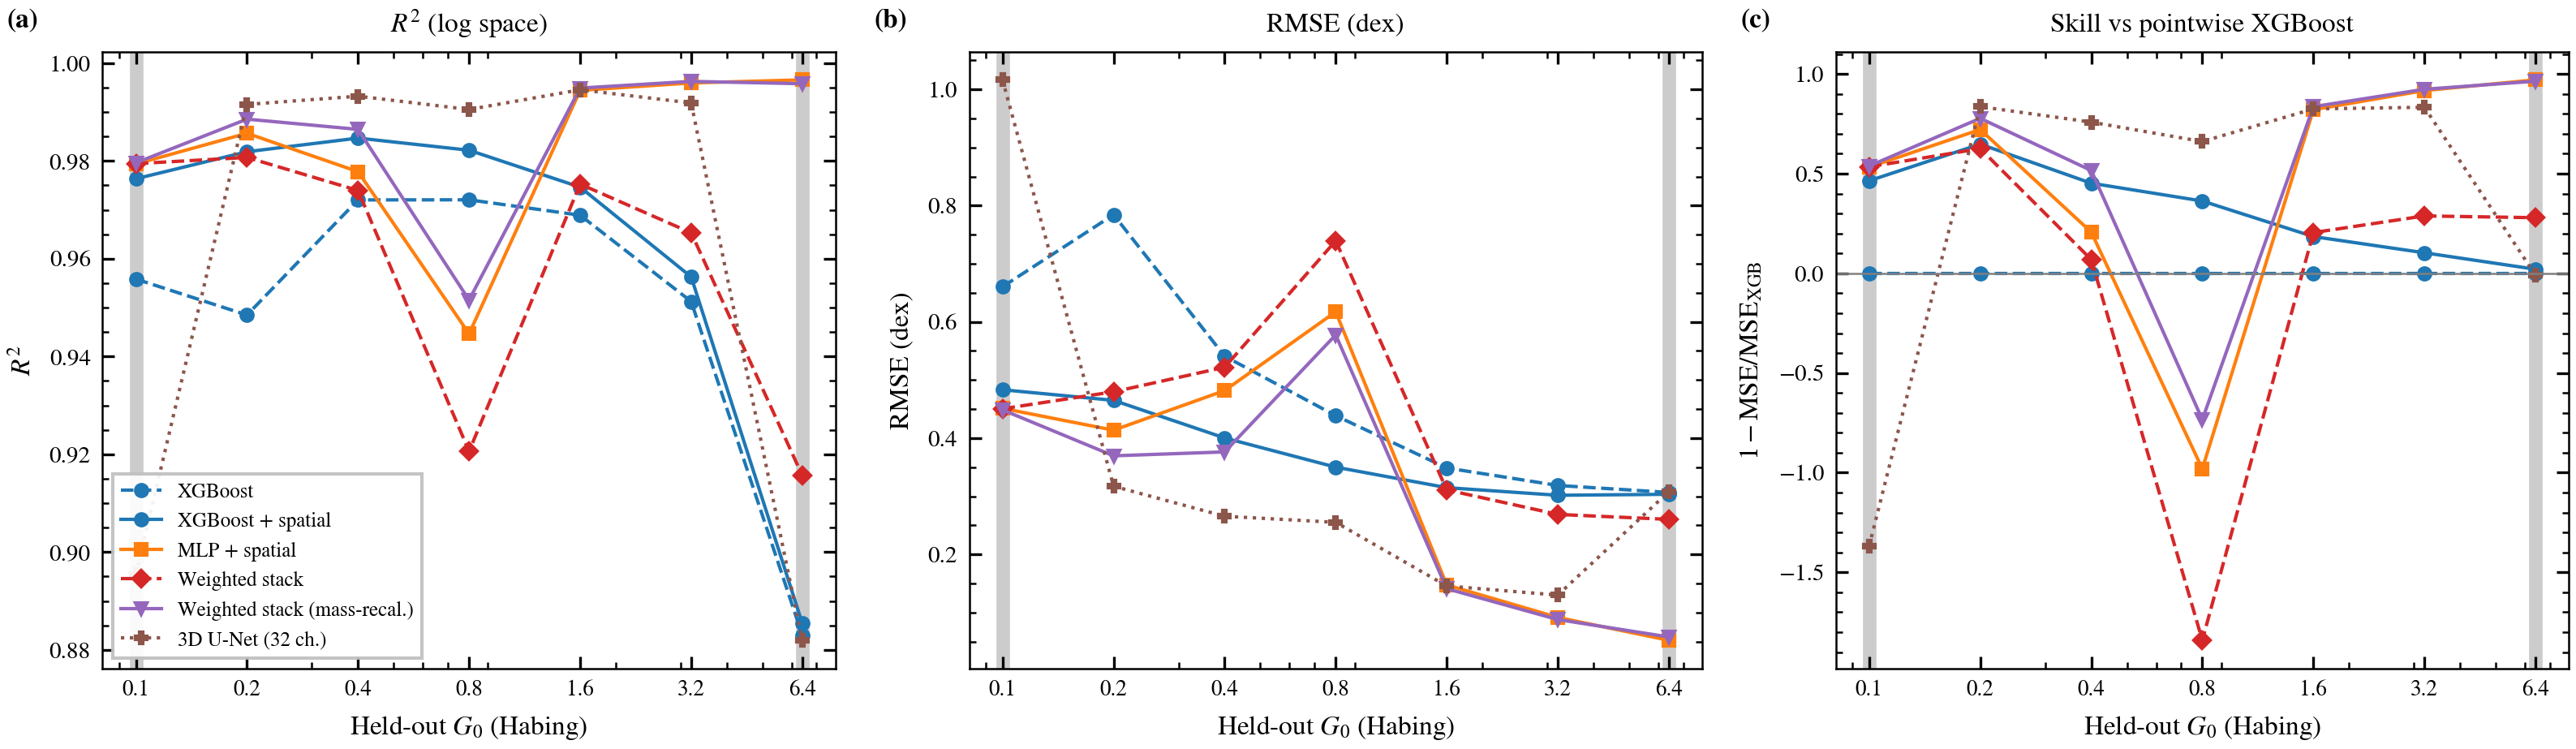
\includegraphics[width=\textwidth]{figures/fig_model_comparison.png}
\caption{Per-fold behaviour across the \(\Gzero\) sweep: log-space
\(\Rsq\) (\emph{a}), RMSE (\emph{b}), and skill against the pointwise
XGBoost baseline (\emph{c}). Grey bands mark the two extrapolation
folds. The 3D U-Net (dotted) is the most accurate model on the interior
folds and the least robust at both boundaries; the mass-calibrated
weighted stack (purple) is the only model that remains strong across
the entire range.}
\label{fig:modelcomp}
\end{figure*}

\subsection{The deployed pipeline}
\label{sec:deployed}

The deployed pipeline --- the density-weighted spatial stack with fully
nested stacking and mass calibration --- reaches per-fold \(\Rsq\) of
0.977--0.998 (mean \(0.990 \pm 0.006\)), RMSE \(0.25\dex\), cell-mean bias
\(+0.02\dex\), total H\(_2\) mass within 0.985--1.090 of truth in
\emph{every} fold, molecular-phase \(\Rsq = 0.979\)--0.994, mass-weighted
MAE \(0.06\dex\), and mean \(W_1 = 0.08\dex\) between predicted and true
marginals (Figure~\ref{fig:massbudget}). The metric-level clip is never
active for these volumes. Residual errors concentrate in the diffuse
UV-exposed gas at low \(\Gzero\), where small shielding-column
differences move cells across the steep atomic-to-molecular transition;
the hardest fold is the \emph{interior} one at \(\Gzero = 0.8\)
(bias \(+0.16\dex\)), a reminder that interpolation folds are not
automatically easy. The full pipeline --- features, training,
calibration, prediction for all seven folds --- runs in about an hour on
one consumer GPU and predicts a new \(128^3\) cube in seconds.

\begin{figure*}
\centering
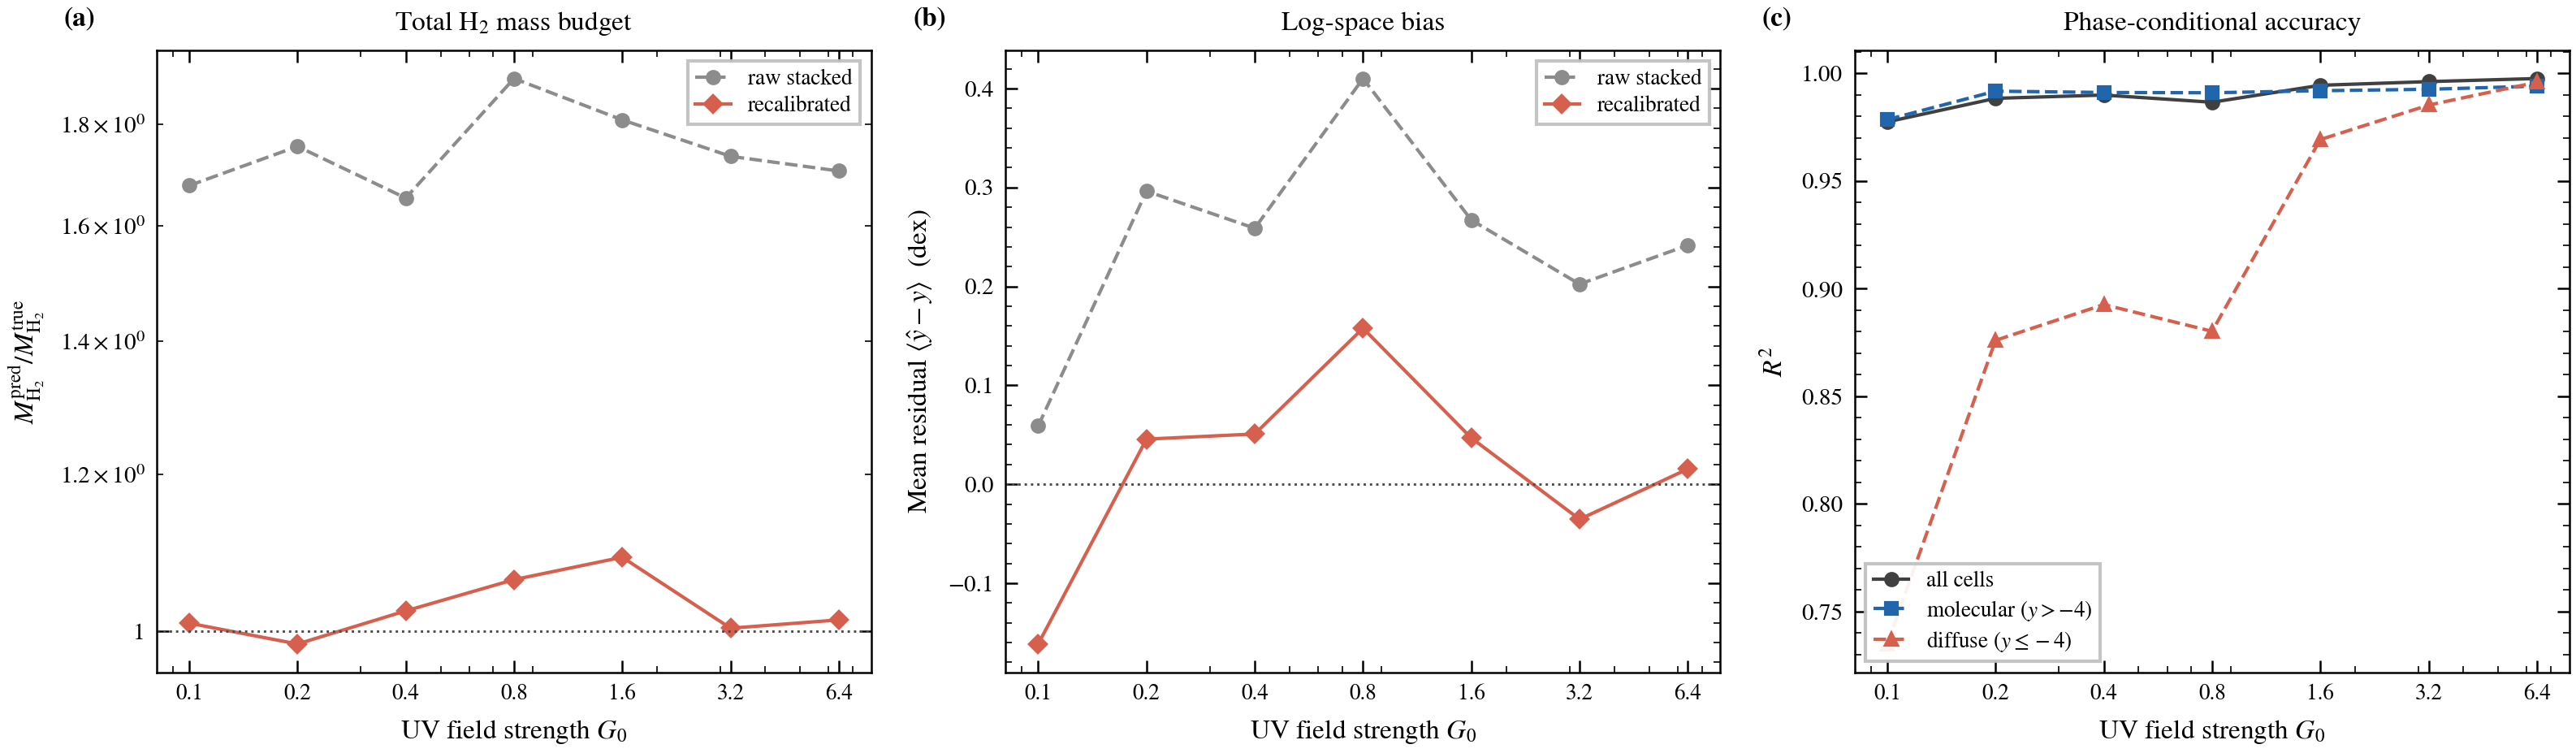
\includegraphics[width=\textwidth]{figures/fig7_massbudget.png}
\caption{The deployed pipeline, per held-out fold. \emph{(a)} Total
H\(_2\) mass ratio: the raw stack (grey) over-predicts by
\(\times\)1.65--1.90 at every \(\Gzero\); the mass-calibrated prediction
(red) is within 9 per cent of the true mass in every fold.
\emph{(b)} Cell-mean log residual. \emph{(c)} Phase-conditional
\(\Rsq\): molecular-phase accuracy is uniformly high; the diffuse phase
is hardest at low \(\Gzero\), where UV-exposed gas spans the steep
atomic-to-molecular transition.}
\label{fig:massbudget}
\end{figure*}

\subsection{The volumetric alternative}
\label{sec:cnn}

The U-Net occupies a revealing position: it is simultaneously the best
interpolator and the least reliable extrapolator. On the five interior
folds it is the most accurate model evaluated (\(\Rsq = 0.992\),
RMSE \(0.22\dex\), against 0.984 and \(0.31\dex\) for the calibrated
stack) --- direct evidence that a learned volumetric representation
extracts non-local information the box filters miss. At the boundaries
the picture inverts: mean edge-fold \(\Rsq\) falls to 0.889
(RMSE \(0.66\dex\)), at \(\Gzero = 0.1\) it is far worse than the
pointwise XGBoost baseline (skill \(-1.37\)), and at \(\Gzero = 6.4\) its
molecular-phase bias is \(+1.13\dex\) with a fold mass ratio above 290
(a lower bound under the clip). Crucially, this failure is not
calibration-repairable: the U-Net's held-out bias is phase-localised
and non-monotonic in \(\Gzero\) (fold mass ratios 1.7, 2.1, 1.1, 0.71,
1.8, 19.0, 291), whereas the stack's bias is a global,
\(\Gzero\)-smooth offset --- the difference between a correctable
systematic and a genuine extrapolation breakdown. The U-Net is also
\(\sim\)5\(\times\) costlier to train than the entire tabular comparison
and, with 48 augmented volumes against millions of parameters,
configuration-sensitive (mean \(\Rsq\) 0.80--0.97 across capacity and
regularisation variants in a dedicated study). We did not pursue
CNN-specific remedies (weighted volumetric losses, bounded outputs,
pretraining), so we make no claim about the ultimate capability of
volumetric architectures; on a suite of this size, engineered spatial
context plus calibration is the robust default, and the volumetric
model is preferable only within a densely sampled parameter range.

\subsection{Dependence on the solver's shielding factor}
\label{sec:ablation}

One input, \(\fshield\), is produced by the solver the surrogate
replaces, so its contribution must be quantified, not assumed. Excluded
from both the local features and the spatial averages, the deployed
configuration retains \(\Rsq = 0.964 \pm 0.014\) with its mass budget
intact (fold ratios 0.93--1.16) --- but its RMSE grows by 60 per cent
(0.29 to \(0.47\dex\)) and the molecular-phase \(\Rsq\) falls from 0.991
to 0.840, reaching 0.70 in the most molecular cube (\(\Gzero = 0.1\)).
The spatial features absorb roughly half of the pointwise models'
ablation loss, consistent with neighbourhood averages of density and
extinction acting as crude column estimators, and XGBoost gain
importance corroborates the picture (\(\log\fshield\) carries 0.57 of
the pointwise gain, 0.83 with its spatial averages; velocity and
magnetic-field components are negligible). The complementary bound
comes from a U-Net trained on 11 chemistry-free inputs (temperature,
\(\Gzero\), velocity, magnetic field): it still reaches
\(\Rsq = 0.851 \pm 0.121\) --- the H\(_2\) \emph{morphology} is largely
inferable from dynamics, thermodynamics, and the UV strength --- but
with \(0.72\dex\) scatter, near-zero molecular-phase \(\Rsq\), and fold
mass ratios from 0.29 to a clipped \(\times\)510. Morphology is cheap;
chemistry is not. Deployable accuracy \emph{inside} the molecular phase
therefore depends on a shielding estimate of \(\fshield\) quality, e.g.\
from extinction or an approximate radiative-transfer sweep.

% ============================================================
\section{Discussion and conclusions}
\label{sec:disc}

The question posed in Section~\ref{sec:intro} has a quantitative
answer: a per-cell surrogate with engineered neighbourhood features,
density-weighted training, and a mass-weighted bias calibration
predicts the \(\nHH\) field of an unseen-\(\Gzero\) simulation with
RMSE \(0.25\dex\), \(\Rsq = 0.990\), and total H\(_2\) mass within 9 per
cent in every fold --- and each of those three ingredients addresses a
distinct error component (scatter, mass placement, bias). Two broader
lessons follow.

First, \emph{scoring determines conclusions}. Ranked by log-space
\(\Rsq\), the raw stack, the calibrated stacks, and the U-Net are
nearly interchangeable (0.959--0.985); ranked by the physical metrics
they span mass errors from 7 per cent to two orders of magnitude. The
bias--scatter decomposition, the mass ratio, and phase-conditional
errors should be standard reporting for field-level emulators
--- and the choice of calibration functional (cell-mean versus
mass-weighted) is a physical decision that changes the recovered mass
by tens of per cent, so it should be stated and, ideally, both variants
reported.

Second, \emph{representation and calibration beat architecture
out-of-distribution}. The spatial features cut tabular RMSE by
23--38 per cent --- several times more than any architecture variation
we tested, consistent with the competitiveness of tree ensembles on
tabular data \citep{Grinsztajn2022} --- while the U-Net's genuine
interpolation advantage does not survive leaving the training range.
For suites of this size the practical division of labour is: engineered
features plus calibration for robust extrapolation; the volumetric
model only within a densely sampled parameter range.

The claims are bounded by the suite's design. The seven simulations
share one turbulent realisation, so generalisation across realisations,
metallicities, dust models, or resolutions is untested; the suite is
quasi-equilibrium and uniformly illuminated; the box-filter features
and the U-Net's zero padding approximate the context of cells near box
faces; and the density-weighting anchors are a designed choice whose
sensitivity we have not mapped. The deployable (no-\(\fshield\))
configuration is a usable surrogate for aggregate statistics and
morphology, but per-cell molecular-phase accuracy requires genuine
shielding information. Within those bounds the result stands: judged as
a physical field, the H\(_2\) density of an unseen UV environment is
predictable --- provided the surrogate is scored, weighted, and
calibrated in physical terms.

% ============================================================
\section*{Acknowledgements}
This work grew out of a final project for the course \emph{Selected
Topics in Robotics and AI} in the Technion Department of Aerospace
Engineering. The author thanks Netanel Ratner for teaching the course
and for giving students the freedom to choose independent final-project
topics. The author thanks Dr Shmuel Bialy of the Technion Department of
Physics for suggesting the project, providing access to the simulation
data, and offering guidance throughout the work. The author also thanks
Ethan Chelly for early brainstorming discussions and for assistance
with the initial CNN exploration.

AI tools were used during the project to assist with code generation
and debugging, exploratory analysis of results, and drafting and
editing of the manuscript. All scientific decisions, interpretation of
results, validation of code outputs, and final manuscript content are
the responsibility of the author.

\section*{Software}

Python 3.14.5; PyTorch 2.12 \citep{Paszke2019}; XGBoost 3.2
\citep{Chen2016}; NumPy 2.4 \citep{Harris2020}; SciPy 1.17
\citep{Virtanen2020}; scikit-learn 1.8 \citep{Pedregosa2011};
Matplotlib 3.10 \citep{Hunter2007}. All experiments were run on a
single NVIDIA GeForce RTX 3090.

\section*{Data availability}

All experiment logs, trained-model outputs, and prediction volumes are
archived as timestamped JSON and \texttt{.npz} files and are available
from the author on request. The simulation suite is not yet public;
requests for data access may be directed to the corresponding author.

% ============================================================
\bibliographystyle{rasti}
\bibliography{references}

\label{lastpage}
\end{document}
